
\section{Monoidal properties}

\subsection{Monoidal functors}

TBW categorically. Induce functor on Monoids.

\subsection{Day convolution}

Define

\subsection{Cubical singular complex}

It is monoidal.


%By definition, the functor of chains $\cchains \colon \cube \to \Ch$ is monoidal, i.e., the diagram
%\begin{equation*}
%\begin{tikzcd}
%2^p \times 2^q \arrow[r, "\cong"] \arrow[d, "\cchains \otimes \cchains"']& 2^{p+q} \arrow[d, "\cchains"] \\
%\cchains(\cube^p) \otimes \cchains(\cube^q) \arrow[r, "\cong"] & \cchains(\cube^{p+q})
%\end{tikzcd}
%\end{equation*}
%commutes and $\cchains(2^0) = R$.

\subsection{Serre coalgebra}

$\cchains$ is monoidal. $\cchainsAS$ is monoidal

%The lift of  $N \colon \cube \to \Ch$ to the symmetric monoidal category $\coAlg$ is also monoidal since the following diagrams associated to the Serre diagonal and augmentation map commute:
%\begin{equation*}
%\begin{tikzcd}
%\cchains(\cube^p) \otimes \cchains(\cube^{q}) \arrow[r, "\cong"] \arrow[d, "(23) \circ (\Delta \otimes \Delta)"'] & \cchains(\cube^{p+q}) \arrow[d, "\Delta"]\\
%\cchains(\cube^p)^{\otimes 2} \otimes \cchains(\cube^{q})^{\otimes 2} \arrow[r, "\cong"]& \cchains(\cube^{p+q})^{\otimes 2}
%\end{tikzcd}
%\qquad \qquad
%\begin{tikzcd}
%\cchains(\cube^p) \otimes \cchains(\cube^{q}) \arrow[r, "\cong"] \arrow[d, "(\varepsilon \otimes \varepsilon)"'] & \cchains(\cube^{p+q}) \arrow[d, "\varepsilon"] \\
%R \otimes R \arrow[r, "\cong"] & R.
%\end{tikzcd}
%\end{equation*}

\subsection{Equivariance of the Serre coproduct}
%We will use the following observation about the Serre diagonal to define the Hopf structure on $\M$.
There is an action of $\S_n$ on $\chains(\cube^n)$ given by permuting the factors of $\chains(\cube^1)^{\otimes n}$.
The Serre diagonal is equivariant with respect to this action in the following sense.

\begin{lemma} \label{l:serre diagonal invariant}
	Let $T$ be the braiding of $\Ch$.
	The following diagram commutes
	\begin{equation*}
	\begin{tikzcd}
	\chains(\cube^1)^{\otimes 2} \arrow[r, "\Delta"] \arrow[d, "T"] &
	\chains(\cube^1)^{\otimes 2} \otimes \chains(\cube^1)^{\otimes 2} \arrow[d, "T \otimes T"] \\
	\chains(\cube^1)^{\otimes 2} \arrow[r, "\Delta"] &
	\chains(\cube^1)^{\otimes 2} \otimes \chains(\cube^1)^{\otimes 2}.
	\end{tikzcd}
	\end{equation*}
\end{lemma}

\begin{proof}
	This can be proven by a straightforward verification. Conceptually, it holds because $(12)(34)(23) = (23)(13)(24)$ in $\S_4$.
\end{proof}

\subsection{Hopf operads}

So far we have consider operad and props over the category $\Ch$ but, since $\coAlg$ is also a symmetric monoidal category, we can consider them over $\coAlg$ as well.
That is to say, demand that all defining chain complexes be coalgebras with composition maps being morphisms of coalgebras.
We refer to operads and props over $\coAlg$ as \textit{Hopf operads and props} respectively.

If $\O$ is a Hopf operad, the category $\coAlg_\O$ is monoidal with structure maps of a product of $\O$-coalgebras $C \otimes C^\prime$ given by
\begin{equation*}
\begin{tikzcd} [column sep = normal, row sep=large]
\O(r) \otimes (C \otimes C^\prime) \arrow[r, "\Delta_\O \otimes \id"] &[10 pt] \O(r) \otimes \O(r) \otimes (C \otimes C^\prime) \arrow[d, "Sh"'] & & \\ &
\big(\O(r) \otimes C \big) \otimes \big( \O(r) \otimes C \big) \arrow[r] & 
C^{\otimes r} \otimes C^{\prime\, \otimes r} \arrow[r, "Sh"] &
(C \otimes C^\prime)^{\otimes r}.
\end{tikzcd}
\end{equation*}
A similar statement holds for the category of representations of a Hopf prop.

\subsection{Cubical structure on $\M$}


------------------

%\section{The prop $\M$}

\subsection{Operads and props} \label{s:operads and props}

Let $\S$ be the category whose objects are the natural numbers and whose set of morphisms between $m$ and $n$ is empty if $m \neq n$ and is otherwise the symmetric group $\S_n$.
A \textit{left $\S$-module} (resp. \textit{right} $\S$-\textit{module} or $\S$-\textit{bimodule}) is a covariant functor from $\S$ (resp. $\S^\op$ or $\S \times \S^\op$) to $\Ch$.
In this paper we prioritize left module structures over their right counterparts. As usual, taking inverses makes both perspectives equivalent.
We respectively denote by $\smod$ and $\sbimod$ the categories of left $\S$-modules and of $\S$-bimodules with morphisms given by natural transformations.

The collections of group homomorphism $\S_n \to \S_n \times \S_1$ for $n \geq 0$ induces a forgetful functor $U \colon \sbimod \to \smod$.
The similarly defined forgetful functor to right $\S$-modules will not be used.

Given an object $C$ in $\C$ define:
\begin{align*}
\End^C(r) &= \Hom(C, C^{\otimes r}),
&\End^C_C(r, s) &= \Hom(C^{\otimes r}, C^{\otimes s}),
\end{align*}
with their natural structures of $\S$-module and $\S$-bimodule respectively.
The forgetful functor $U$ sends $\End^C_C$ to $\End^C$.

We can define \textit{operads} and \textit{props} by enriching $\S$-modules and \mbox{$\S$-bimodules} with certain composition structures.
For a complete presentation of these concepts we refer to Definition 11 and 54 of \cite{Markl08}.
Intuitively, operads and props can be understood by abstracting the composition structure naturally present in the left $\S$-module $\End^C$, naturally an operad, and the $\S$-bimodule $\End^C_C$, naturally a prop.
We remark that the structure on a prop $\P$ restricts to an operad structure on $U(\P)$.

We can also think of operads and props as algebras over the monad associated to the free-forgetful adjunctions
\begin{equation*}
\begin{tikzcd}
\smod \arrow[r, bend left] & \arrow[l, bend left] \operads 
& \text{and} &
\sbimod \arrow[r, bend left] & \arrow[l, bend left] \props
\end{tikzcd}
\end{equation*}
which we now review, see \cite{markl2008props} or \cite{fresse2010props} for a more detailed presentation.

The \textit{free prop} $F(M)$ generated by an \mbox{$\S$-bimodule} $M$ is constructed using open directed graphs with no directed loops that are enriched with a labeling described next. We think of each directed edge as built from two compatibly directed half-edges. For each vertex $v$ of a directed graph $G$, we have the sets $in(v)$ and $out(v)$ of half-edges that are respectively incoming to and outgoing from $v$. Half-edges that do not belong to $in(v)$ or $out(v)$ for any $v$ are divided into the disjoint sets $in(G)$ and $out(G)$ of incoming and outgoing external half-edges. For any positive integer $n$ let $\overline{n} = \{1,\dots,n\}$ and set $\overline{0} = \emptyset$. For any finite set $S$, denote the cardinality of $S$ by $|S|$. The labeling is given by bijections  
\begin{equation*}
\overline{|in(G)|}\to in(G), \qquad
\overline{|out(G)|}\to out(G),
\end{equation*}
and
\begin{equation*}
\overline{|in(v)|}\to in(v), \qquad
\overline{|out(v)|}\to out(v),
\end{equation*}
for every vertex $v$.
We refer to the isomorphism classes of such labeled directed graphs with no directed loops as $(n,m)$\textit{-graphs} denoting the set of these by $\G(m,n)$.
We use graphs immersed in the plane to represent elements in $\G(m,n)$, please see Figure \ref{f:immersion}.
We consider the right action of $\S_n$ and the left action of $\S_m$ on a $(n,m)$-graph given respectively by permuting the labels of $in(G)$ and $out(G)$. This action defines the $\S$-bimodule structure on the free prop
\begin{equation} \label{e:free prop}
F(M)(m,n) \ = \bigoplus_{\Gamma \in \G(m,n)} \bigotimes_{v \in Vert(\Gamma)} out(v) \otimes_{\S_q} M(p, q) \otimes_{\S_p} in(v),
\end{equation}
where we simplified the notation writing $p$ and $q$ for $\overline{|in(v)|}$ and $\overline{|out(v)|}$ respectively. The composition structure is defined by (relabeled) grafting and disjoint union.
The free operad is constructed similarly only using $(1,m)$-graphs.

Let us now focus on the category $\Ch$.
Let $C$ be a chain complex, $\O$ an operad, and $\P$ a prop.
An $\O$-\textit{coalgebra} (resp. $\O$-\textit{algebra} or $\P$-\textit{bialgebra}) structure on $C$ is a structure preserving morphism $\O \to \End^C$ (resp. $\P \to \End_C^C$).

An $\S$-module $M$ is said to be $E_\infty$ if for each $r$ the chain complex $M(r)$ is an algebraic model for the universal bundle $E\S_r$, i.e., it is free as an $\S_r$-module and its homology is that of a point.
An operad is said to be $E_\infty$ if its underlying $\S$-modules is $E_\infty$.
A prop $\P$ is said to be $E_\infty$ if $U(\P)$ is an $E_\infty$ operad.

\begin{figure}
	\begin{tikzpicture}[scale=.6]
\draw (1,3.7) to (1,3); 

\draw (1,3) to [out=205, in=90] (0,0);

\draw [shorten >= 0cm] (.6,2.73) to [out=-100, in=90] (2,0);

\draw [shorten >= .15cm] (1,3) to [out=-25, in=30, distance=1.1cm] (1,1.5);
\draw [shorten <= .1cm] (1,1.5) to [out=210, in=20] (0,1);

\node at (1,3.9){};
\node at (0,-.32){};
\node at (2,-.32){};

\node at (3,1.5){$\sim$\ \ \ };
\end{tikzpicture}
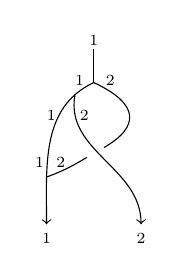
\begin{tikzpicture}[scale=.6]
\draw (1,3.7) to (1,3); 

\draw [->](1,3) to [out=205, in=90] (0,0);

\draw [shorten >= 0cm,->] (.6,2.73) to [out=-100, in=90] (2,0);

\draw [shorten >= .15cm] (1,3) to [out=-25, in=30, distance=1.1cm] (1,1.5);
\draw [shorten <= .1cm] (1,1.5) to [out=210, in=20] (0,1);


\def\x{.8}

\node[scale=\x] at (1,3.9){$\scriptstyle 1$};

\node[scale=\x] at (.7,3.05){$\scriptstyle 1$};
\node[scale=\x] at (1.35,3.05){$\scriptstyle 2$};

\node[scale=\x] at (.1,2.3){$\scriptstyle 1$};
\node[scale=\x] at (.8,2.3){$\scriptstyle 2$};

\node[scale=\x] at (-.15,1.3){$\scriptstyle 1$};
\node[scale=\x] at (.3,1.3){$\scriptstyle 2$};

\node[scale=\x] at (0,-.3){$\scriptstyle 1$};
\node[scale=\x] at (2,-.3){$\scriptstyle 2$};
\end{tikzpicture}
	\caption{Immersed graphs represent labeled directed graphs with the direction implicitly given from top to bottom and the labeling from left to right.}
	\label{f:immersion}
\end{figure}

\subsection{The prop $\M$}\label{propM}

Let us consider the free prop $F(N)$ generated by the $\S$-bimodule $N$ whose only non-zero chain complexes are concentrated in degree $0$ and are give by
\begin{equation*}
N(1, 0) = R\{\varepsilon\}, \qquad
N(1, 2) = R[\S_2]\{\Delta\}.
\end{equation*}
Define $\As$ as the quotient of $F(N)$ by the prop ideal generated by the relations
\begin{equation*}
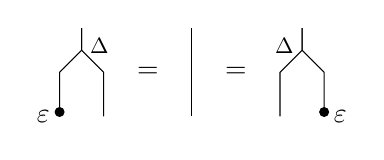
\begin{tikzpicture}[scale=.28]
\draw (-4,0)--(-4,2)--(-5,3)--(-5,4);
\draw (-6,0)--(-6,2)--(-5,3)--(-5,4);
\node [scale=.8] at (-4.2,3.2) {$\Delta$};
\draw [fill] (-6,.2) circle [radius=.2];
\node [left] at (-6,0) {$\varepsilon$};

\node at (-2,2) {=};
\draw (0,0)--(0,4);
\node at (2,2) {=};

\draw (4,0)--(4,2)--(5,3)--(5,4);
\draw (6,0)--(6,2)--(5,3)--(5,4);
\node [scale=.8] at (4.2,3.2) {$\Delta$};
\draw [fill] (6,.2) circle [radius=.2];
\node [right] at (6,0) {$\varepsilon$};
\end{tikzpicture}
\qquad \qquad
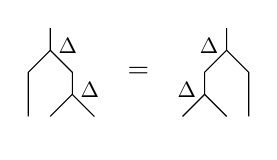
\begin{tikzpicture}[scale=.28]
\node at (0,2){=};
\node at (0,0) {\phantom{$\varepsilon$}};

\draw (2,0)--(3,1)--(3,2)--(4,3)--(4,4);
\draw (4,0)--(3,1);
\draw (4,3)--(5,2)--(5,0);
\node [scale=.8] at (3.2,3.2) {$\Delta$};
\node [scale=.8] at (2.2,1.2) {$\Delta$};

\draw (-2,0)--(-3,1)--(-3,2)--(-4,3)--(-4,4);
\draw (-4,0)--(-3,1);
\draw (-4,3)--(-5,2)--(-5,0);
\node [scale=.8] at (-3.2,3.2) {$\Delta$};
\node [scale=.8] at (-2.2,1.2) {$\Delta$};
\end{tikzpicture}
\end{equation*}
We remark that the category $\coAlg_{U(\As)}$ is equivalent to $\coAlg$.

Let $W^{(1)}$ be the chain complex of free $R[\S_2]$-modules
\begin{equation*}
\begin{tikzcd}
R[\S_2]\{\nu\} &[0pt] \arrow[l, "1-T"'] R[\S_2]\{\mu\},
\end{tikzcd} 
\end{equation*}
which is isomorphic to the cellular chains on the standard $\S_2$-equivariant $CW$-structure on the circle
\begin{equation*}
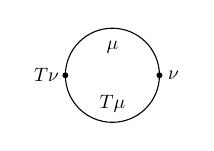
\begin{tikzpicture}[scale=.85]
\draw (0,0) circle (20pt);
\node[scale=.7] at (0,12pt){$\mu$};
\node[scale=.7] at (0,-12pt){$T \mu$};
\node[scale=.7] at (-28pt,0){$T \nu$};
\node[scale=.7] at (26pt,0){$\nu$};
\draw [fill] (-20pt,0) circle [radius=1pt];
\draw [fill] (20pt,0) circle [radius=1pt];
\end{tikzpicture}
\end{equation*}
and let $W^{(0)}$ be the subcomplex generated by $\nu$. We think of $W^{(1)}$ as an $\S_2$-equivariant 1-cell with boundary $W^{(0)}$.

We regard these complexes as $\S$-bimodules concentrated in biarity $(2,1)$, and let $\varphi \colon W^{(0)} \to \As$ be define by sending $T \nu$ and $\nu$ respectively to
\begin{equation*}
\begin{tikzpicture}[scale=.2]
\draw (-4,0)--(-4,4);
\draw (-6,0)--(-6,4);
\draw [fill] (-6,.2) circle [radius=.2];
\node [left] at (-6,0) {$\varepsilon$};

\node at (0,.4) {and};

\draw (4,0)--(4,4);
\draw (6,0)--(6,4);
\draw [fill] (6,.2) circle [radius=.2];
\node [right] at (6,0) {$\varepsilon$.};
\end{tikzpicture}
\end{equation*}
Consider the push-out
\begin{equation*}
\begin{tikzcd}
F(W^{(0)}) \arrow[r, "F(\varphi)"] \arrow[d] & \As \arrow[d, dashed] \\
F(W^{(1)}) \arrow[r, dashed] & \mu \vee_\varphi \As
\end{tikzcd}
\end{equation*}
in the category of props. We think of $\mu \vee_\varphi \As$ as the prop obtained by attaching a $1$-cell in biarity $(2,1)$ to $\As$.

Define $\M$ as the quotient of $\mu \vee_\varphi \As$ by the ideal generated by
\begin{equation*}
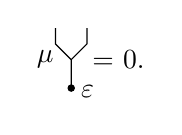
\begin{tikzpicture}[scale=.2]
\draw (5,4)--(5,3)--(6,2)--(6,0);
\draw (7,4)--(7,3)--(6,2);
\node [left] at (5.5,2) {$\mu$};
\draw [fill] (6,.2) circle [radius=.2];
\node [right] at (6,0) {$\varepsilon$};

\node at (9,2) {= 0.};
\end{tikzpicture}
\end{equation*}

We can give a more explicit description of $\M$ using the description of the free prop in terms of $(m,n)$-graphs.
Consider the following elements in $\M$
\begin{equation*}
\counit \in \mathcal M(1,0)_0, \hspace*{.6cm} \coproduct \in \mathcal M(1,2)_0, \hspace*{.6cm} \product \in \mathcal M(2,1)_1,
\end{equation*}
where the decorations by $\varepsilon$, $\Delta$, and $\mu$ are omitted.
Any element in $\M(m,n)$ can be written as a linear combination of the $(m,n)$-graphs generated by these three by grafting, disjoint union and relabeling, modulo the ideals generated by the relations
\begin{equation*}
\qquad \leftcounitality \, , \qquad \rightcounitality \, , \qquad \coassociativity \, , \qquad \productcounit \, .
\end{equation*}
Its chain complex structure is determined using \eqref{e:free prop} by 
\begin{equation*}
\partial\ \counit = 0, \hspace*{.6cm} \partial \ \coproduct = 0, \hspace*{.6cm} \partial \ \product = \ \boundary \, .
\end{equation*}

The following result was shown in \cite{Medina20prop1}.

\begin{proposition}
	The prop $\M$ is an $E_\infty$-prop.
\end{proposition}

Since $\As$ includes into $\M$, there is a functor between the corresponding categories of coalgebras $\coAlg_{U(\M)} \to \coAlg_{U(\As)} = \coAlg$.



---------------
As can be seen from \eqref{e:free prop}, the $(m,n)$-part of the free prop is defined only up to a choice of total order on the set of vertices of the $(m,n)$-graph involved.

\begin{definition}
	Let $\Gamma \in \G(m,n)$ be a representative of an element in $\M(m,n)$ of degree $d$. A \textit{characteristic map} for $\Gamma$ is the chain map \vspace*{-5pt}
	\begin{equation} \label{e:order chain map}
	\begin{tikzcd}[row sep=tiny, column sep=small]
	\iota_\Gamma \colon \cchains(\square^d) \arrow[r] & \M(m,n) \\
	\qquad {[0,1]}^{\otimes d} \arrow[r, |->] & \Gamma.
	\end{tikzcd}
	\end{equation}
	induced by a choice of total order of the vertices of $\Gamma$.
\end{definition}


\subsection{Hopf structure on $\M$}

In this subsection we show that $\M$ is a Hopf prop, that is, a prop over the category $\coAlg$.

Since, by Lemma~\ref{l:serre diagonal invariant}, the Serre diagonal is equivariant, the following is well-defined.
\begin{definition}
	For any $(m,n)$ the \textit{coproduct} $\Delta_\M(m,n) \colon \M(m,n) \to \M(m,n)^{\otimes 2}$ is defined on a basis element $\Gamma$ by
	\begin{equation} \label{e:diagonal of M}
	\Delta_{\M}(\Gamma) = \iota_\Gamma^{\otimes 2} \circ \Delta \left([0,1]^{\otimes d}\right)
	\end{equation}
	where $\iota_\Gamma$ is a characteristic map of $\Gamma$ and $\Delta$ is the Serre diagonal.
	The \textit{counit} $\varepsilon_\M(m,n) \colon \M(m,n) \to R$ is the chain map whose value on basis elements of degree $0$ is $1$. 
\end{definition}

\begin{theorem}
	The collections of maps $\Delta_\M = \{\Delta_\M(m,n)\}_{m,n \geq 0}$ and $\varepsilon_\M = \{\varepsilon_\M(m,n)\}_{m,n\geq0}$ make $\M$ into a Hopf prop, i.e., a prop over the category $\coAlg$.
\end{theorem}

\begin{proof}
	The collection of maps $\Delta_\M$ are compatible with the composition structure on $\M$ since given characteristic maps $\iota_\Gamma$ and $\iota_{\Gamma^\prime}$,  $\iota_\Gamma \otimes \iota_{\Gamma^\prime}$ is a characteristic map of any (vertical or horizontal) composition of $\Gamma$ and $\Gamma^\prime$.
	It respects the relations defining $\M$ since
	\begin{center}
		\begin{tikzcd}
		\leftcounitcoproduct \arrow[r, "\Delta_\M"] \arrow[d, <->] &[-0pt] \leftcounitcoproduct \otimes \leftcounitcoproduct \arrow[d, <->] \\
		\identity \arrow[r, "\Delta_\M"] & \ \, \identity \otimes \identity \, ,
		\end{tikzcd}
		\qquad
		\begin{tikzcd}
		\rightcounitcoproduct \arrow[r, "\Delta_\M"] \arrow[d, <->] &[-0pt] \rightcounitcoproduct \otimes \rightcounitcoproduct \arrow[d, <->] \\
		\identity \arrow[r, "\Delta_\M"] & \ \, \identity \otimes \identity \, ,
		\end{tikzcd}
		\qquad
		\begin{tikzcd}
		\leftcomb \arrow[r, "\Delta_\M"] \arrow[d, <->] &[-0pt] \leftcomb \, \otimes \leftcomb \arrow[d, <->] \\
		\rightcomb \arrow[r, "\Delta_\M"] & \, \rightcomb \, \otimes \rightcomb,
		\end{tikzcd}
		\qquad
		\begin{tikzcd}
		\productcounit \arrow[r, "\Delta_\M"] \arrow[d, <->] &[-0pt] \counit\ \counit \, \otimes \productcounit + \productcounit \otimes \, \counit\ \counit \arrow[d, <->] \\
		0 \arrow[r, "\Delta_\M"] & \ 0.
		\end{tikzcd}
	\end{center}
	It is a chain map since
	\begin{center}
		\begin{tikzcd}
		\counit \arrow[r, "\Delta_\M"] \arrow[d, "\partial"'] &[-0pt] \counit \otimes \counit \arrow[d, "\partial"'] \\
		0 \arrow[r, "\Delta_\M"] & \ \, 0 \, ,
		\end{tikzcd}
		\qquad
		\begin{tikzcd}
		\coproduct \arrow[r, "\Delta_\M"] \arrow[d, "\partial"'] &[-0pt] \coproduct \otimes \coproduct \arrow[d, "\partial"'] \\
		0 \arrow[r, "\Delta_\M"] & \ \, 0 \, ,
		\end{tikzcd}
		\qquad
		\begin{tikzcd}
		\product \arrow[r, "\Delta_\M"] \arrow[d, "\partial"'] &[-0pt] \leftboundary \ \otimes \product + \product \otimes\ \rightboundary \arrow[d, "\partial"'] \\
		\rightboundary \,-\, \leftboundary \arrow[r, "\Delta_\M"] &
		\, \rightboundary \otimes \rightboundary \,-\, \leftboundary \otimes \leftboundary\,.
		\end{tikzcd}
	\end{center}
	The compatibility of the collection of maps $\varepsilon_\M$ is checked similarly.
\end{proof}

\subsection{Monoidal $E_\infty$ structures}

We now show the functor $\cchainsUM$ is monoidal.
\begin{theorem} \label{chainsismonoidal}
	The functor $\cube \to \biAlg_{\M}$ of Proposition~\ref{thm: cubical chain bialgebra} is monoidal.
\end{theorem}

\begin{proof}
	We have already establish that the Serre diagonal and the augmentation map are compatible with the monoidal structure of $\cube$. In diagrammatic terms,
	\begin{equation*}
	\begin{tikzcd}
	\coproduct \otimes \chains(\cube^{p+q}) \arrow[r, "\Delta_\M \otimes Sh"] \arrow[d] &[20pt]
	\left( \ \coproduct \otimes \coproduct \ \right) \otimes
	\chains(\cube^{p}) \otimes \chains(\cube^{q}) \arrow[d] \\
	\chains(\cube^{p+q})^{\otimes 2} \arrow[r, "Sh"] &
	\chains(\cube^{p})^{\otimes 2} \otimes \chains(\cube^{q})^{\otimes 2}
	\end{tikzcd}
	\end{equation*}
	and
	\begin{equation*}
	\begin{tikzcd}
	\counit \ \otimes \chains(\cube^{p+q}) \arrow[r, "\Delta_\M \otimes Sh"] \arrow[d] &[20pt]
	\left( \ \counit \ \otimes \ \counit \ \right) \otimes
	\chains(\cube^{p}) \otimes \chains(\cube^{q}) \arrow[d] \\
	R \arrow[r, "\cong"] &
	R \otimes R
	\end{tikzcd}
	\end{equation*}
	commute.
	We will now show that the following diagram commutes:
	\begin{equation*}
	\begin{tikzcd}
	\product \otimes \chains(\cube^{p+q})^{\otimes 2} \arrow[d] \arrow[r, "\Delta_\M \otimes Sh"] &[20pt]
	\left(\, \ \leftboundary \ \otimes \product + \product \otimes \ \rightboundary \ \, \right) \otimes \chains(\cube^{p})^{\otimes 2} \otimes \chains(\cube^{q})^{\otimes 2} \arrow[d]\\
	\chains(\cube^{p+q}) \arrow[r, "Sh"] &
	\, \chains(\cube^{p}) \otimes \chains(\cube^{q}).
	\end{tikzcd}
	\end{equation*}
	Since this is immediate for $p=0$ or $q=0$ and $\cube$ is generated as a monoidal category by $2^1$, we only need to verify the commutativity of this diagram for $p=q=1$.
	Consider $(x_1 \otimes y_1) \otimes (x_2 \otimes y_2) \in \chains(\cube^1)^{\otimes 2} \otimes \chains(\cube^1)^{\otimes 2}$.
	We have
	\begin{equation*}
	\begin{split}
	\big((\id \otimes \varepsilon) \otimes \ast \ + \ \ast \otimes (\varepsilon \otimes \Delta)\big) \ (-1)^{\bars{y_1} \bars{x_2}} \ (x_1 \otimes x_2) \otimes (y_1 \otimes y_2) \ & = \\
	(-1)^{\bars{y_1} \bars{x_2} + \bars{x_1} + \bars{x_2} + \bars{y_1}} \ x_1 \cdot \varepsilon(x_2) \otimes y_1 \ast y_2 \ & + \ 
	(-1)^{\bars{y_1} \bars{x_2} + \bars{x_1}} \ x_1 \ast x_2 \otimes \varepsilon(y_1) \ast y_2.
	\end{split}
	\end{equation*}
	The first summand on the left hand side is non-zero only if $\bars{x_2} = \bars{y_1} = \bars{y_2} = 0$, whereas the second is non-zero only if $\bars{x_1} = \bars{x_2} = \bars{y_1} = 0$, so the above is also equal to
	\begin{equation} \label{e:join is monoidal 1}
	(-1)^{\bars{x_1}} \ x_1 \cdot \varepsilon(x_2) \otimes y_1 \ast y_2 \ + \ 
	x_1 \ast x_2 \otimes \varepsilon(y_1) \ast y_2.
	\end{equation}
	On the other hand,
	\begin{align*}
	(x_1 \otimes y_1) \ast (x_2 \otimes y_2) \ & =\ 
	(-1)^{\bars{x_1} + \bars{y_1}} \ (x_1 \ast x_2) \otimes \varepsilon(y_1) \cdot y_2 \ +\
	(-1)^{\bars{x_1} + \bars{y_1}} \ x_1 \cdot \varepsilon(x_2) \otimes (y_1 \ast y_2) \\ \ & =\ 
	(x_1 \ast x_2) \otimes \varepsilon(y_1) \cdot y_2 \ +\
	(-1)^{\bars{x_1}} \ x_1 \cdot \varepsilon(x_2) \otimes (y_1 \ast y_2),
	\end{align*}
	which is equal to \eqref{e:join is monoidal 1} as claimed.
\end{proof}

We have the following immediate consequence.

\begin{theorem} \label{t:lift chains on cSet to UM coAlg is monoidal}
    The functor $\cchainsUM \colon \cSet \to \coAlg_\UM$ is monoidal.
\end{theorem}